\chapter{Literature study}
\section{Overview of DIC and DVC}
DIC and DVC are techniques which quantify the optical flow between images then relate the optical flow observed to displacements in the 3D world. Optical flow is the apparent motion of an object in an image caused by the actual motion of the object in the 3D world.

Thus these techniques solve two problems in order to determine displacements of 3D objects from image of the 3D objects. The first problem is determining the optical flow that is present between images. This is determined by identifying a unique pattern contained within a cluster of pixels, with these pixels representing a part  of the 3D object, in the reference image and finding the same pattern within a cluster of pixels in the deformed image. Then the difference in position of these pixel clusters within the two images can be used to determine the displacement that this part of the 3D object underwent. Note that at this stage the displacement is in units of pixels. 

This process is referred to as correlation. The correlation techniques focused on in this project use gradient-descent methods to determine the location of a pixel cluster, in the deformed image, that matches a cluster in the reference image. Additionally since they rely on tracking pixel clusters, called subsets, these algorithms are referred to as gradient-descent, subset based DIC and DVC.

The second problem to be solved is relating the displacement in units of pixels to the actual displacement in the 3D world in metric units. In order to do this a method of mathematically relating the 2D information stored within an image to the 3D scene that it captures is needed. This mathematical relation is well known and is discussed in section \ref{sec:coord sys}. The actual problem is to determine the value of the parameters that are involved in this mathematical equation. These are solved for by relating the known coordinates of a 3D object to the coordinates of the object within the image using this mathematical relation and solving for the parameters. This is an inverse problem and this process is referred to as calibration. Calibration also has to take into account distortions caused by the camera.

Therefore two image sets are required in order to perform DIC or DVC analysis. The first image set contains images of an object of known coordinates such that the calibration process can be performed. The second image set must contain images taken of an object as it is being deformed or displaced so that these images can be used for correlation.

\section{Correlation}
DIC is used in material science to determine the displacements that the surface of a test specimen experiences when it is deformed by an applied load. First pictures of the speckle pattern applied to the surface of the specimen are taken before and after deformation. Then a cluster of pixels that contains a unique pattern in the reference image is identified and the same pattern in a cluster of pixels is found within the deformed image. By comparing the position of this unique pattern in the reference image to its position in the deformed image the displacement of the pattern can be determined.

The cluster of pixels is referred to as a subset. A subset is used instead of individual pixels because a single pixel in the reference image is likely to have multiple matches in the deformed image since any pixel with the same grayscale value in the deformed image is a possible match. Therefore a subset of pixels is used since it contains more information and is therefore more likely to contain a unique pattern that can be more definitively identified in the deformed image.

% The correlation process involves finding a pattern from one image within another image. In doing so the displacement and deformation that the pattern underwent are determined. Patterns are tracked instead of individual pixels since pixels only contain a grayscale value and thus are not unique within the image. Therefore a pixel in one image could be matched to several pixels in another image since these pixels just need to have the same grayscale value. Generally a cluster of pixels referred to as a subset is identified in the base image and the second image is searched for a subset containing the same pattern.

% Different applications that make use of this correlation process have different requirements. Within material science specifically the displacements \todo{and deformations?} need to be tracked to a very high resolution. For example to create an accurate stress-strain curve for common engineering materials a resolution on the order of $10^{-5} m/m$ is required \cite{sutton2009image}.

\subsection{Correspondence problem and speckle patterns}
Although subsets of pixels are usually easier to track than individual pixels, using subsets leads to a new issue. The correspondence problem is to do with the inability to track displacements as a result of the grayscale patterns within the image. To understand this consider the aperture problem which is a special case of the correspondence problem.

The aperture problem involves the ambiguity in attempting to track the motion of a one-dimensional spatial structure (such as a line) when viewed through an aperture (such as when considering a subset of pixels) that cuts off the view of the ends of the one-dimensional spatial structure \cite{apertureProblem}. This can be illustrated by considering the difficulty in tracking the motion of a line in the direction along the line when the end points of the line are not visible. \todo{image?}

Similarly if the pattern in the image to be tracked is a repeating pattern with a constant grid spacing then the displacement cannot be uniquely determined since the image will contain the same pattern repeated. Thus the algorithm will determine the displacement to be within a multiple of the grid spacing from the actual displacement unless the subset contains a unique feature such as being at the edge of the specimen.

\todo[inline]{deformation and difficulty in tracking edges?}

Thus it is clear that the patterns to be tracked in the images can have a significant impact on the performance of the correlation process. To avoid the aperture problem is is clear that the pattern should be isotropic such that it can be tracked equally well in all directions. Additionally to solve the correspondence problem the pattern should also be highly random and non-periodic so that each subset of an image contains a unique pattern. 

This is achieved by applying a random speckle pattern to the surface of the specimen to be tested since these provide very unique patterns which are isotropic in nature. Additionally the high information density enables smaller subsets to be used than would otherwise have been possible.

% \subsubsection{Correspondence problem and speckle patterns}
% A major problem that can occur when attempting to track patterns in images is the correspondence problem. The correspondence problem has to do with the inability to track displacements in images as a result of the patterns that are available for tracking. To understand this consider the aperture problem which is a special case of the correspondence problem.

% The aperture problem involves the ambiguity in attempting to track the motion of a one-dimensional spatial structure (such as a line) when viewed through an aperture that cuts off the view of the ends of the one-dimensional spatial structure \cite{apertureProblem}. This can be illustrated by considering the difficulty in tracking the motion of a line in the direction along the line when the end points of the line are not visible. \todo{image?}

% Similarly if the pattern in the image to be tracked is a repeating pattern with a constant grid spacing then the displacement cannot be uniquely determined since the image will contain the same pattern repeated. Thus the algorithm will determine the displacement to be within a multiple of the grid spacing from the actual displacement unless the subset contains a unique feature such as being at the edge of the specimen.

% \todo[inline]{deformation and difficulty in tracking edges?}

% Thus it is clear that the patterns to be tracked in the images can have a significant impact on the performance of the correlation process. To avoid the aperture problem is is clear that the pattern should be isotropic such that it can be tracked equally well in all directions. Additionally to solve the correspondence problem the pattern should also be highly random and non-periodic so that each subset's pattern is unique. This is achieved by applying a random speckle pattern to the surface of the specimen to be tested since these provide very unique patterns which are isotropic in nature. Additionally the high information density enables smaller subsets to be used than would otherwise have been possible.

\subsection{Interpolation}
Different applications of DIC place different requirements on the DIC algorithm. Within material science applications one of the main requirements is that the displacements be tracked accurately to a very high resolution. For example to create an accurate stress-strain curve for common engineering materials a resolution on the order of $10^{-5} m/m$ is required \cite{sutton2009image}. This thus requires displacements to be determined to sub-pixel resolutions.

The issue with this is that this requires the light intensity to be continuous whereas digital images are discrete. Interpolation is used to determine the light intensities between pixels so that an approximation to the continuous form of the intensity pattern on the surface of the specimen can be calculated.

\todo[inline]{describe interpolation schemes used: bilinear, bicubic}

\subsection{Warp function}
An additional requirement of applying DIC to material science is that the deformation characteristics of the materials should be taken into account. The deformation of the material causes the speckle pattern on its surface to deform in the same way. This is an issue since the pattern contained within a subset of the reference image will be deformed in the second image which can cause difficulties in matching the two subsets.

This is solved by allowing for the subsets to deform in a similar way to that of the material by defining the allowable deformations in a warp function. The purpose of these warp functions is to transform the pixel coordinates of the reference subset so that the resulting pattern is closer to the pattern in the deformed image. A common warp function which allows for affine transformations is given by
\begin{equation}
	W (\bm{x},\bm{p}) = 
	\begin{bmatrix}
	x_{warp} \\
	y_{warp}
	\end{bmatrix} 
	= \begin{bmatrix}
	x + u + \frac{\partial u}{\partial x} \Delta x + \frac{\partial u}{\partial y} \Delta y \\
	y + v + \frac{\partial v}{\partial x} \Delta x + \frac{\partial v}{\partial y} \Delta y
	\end{bmatrix}.
	\label{eq:warp}
\end{equation}
Here $x$ and $y$ represent the position of the pixel in the original image, $u$ and $v$ represent the displacements in the x and y directions respectively, $\frac{\partial u}{\partial x}$ and $\frac{\partial v}{\partial y}$ represent the elongation in the x and y directions respectively, $\frac{\partial v}{\partial x}$ and $\frac{\partial u}{\partial y}$ represent the shear deformation of the subset, $\Delta x$ and $\Delta y$ are the distances from the centre of the subset to the pixel under consideration and $x_{warp}$ and $y_{warp}$ are the modified pixel coordinates after the warp has been applied.

With most subset based DIC algorithms the more complex the warp function becomes the more computationally expensive each iteration is. This is because the correlation criteria must be optimized in terms of more variables leading to more work.

\subsection{Correlation criteria}
A method of determining how well the reference subset, $G$, has been matched to a subset in the deformed image, $F$, is needed in order for a DIC algorithm to know when correlation has been accomplished. This is done through equations called correlation criteria which describe the fit between the two subsets by a single number. 

Correlation criteria fulfil an additional purpose. As images are taken, as the specimen is deformed, the intensity of the images can change as a result of changes in lighting, changes in reflectivity as the material strains and so on. Although this does not cause the patterns in the subsets to change it does cause the grayscale values of individual pixels, that make up the patterns, to change. Some correlation criteria account for this by accommodating for offset in intensity values or for scaling the intensity values.

Each correlation criteria is based off of a cost function which is usually a variation of the sum of squared differences between the intensities of the reference and investigated subset. They vary in the scaling and offset that is applied to the investigated subset's intensity values. 

\subsubsection{Sum of square difference}
This is one of the more basic correlation criteria since it does not adjust for lighting. It is simply the sum of squared differences between the reference subset and investigated subset.
\begin{equation}
\chi_{SSD}^2 (G) = \sum_{i} \left( G_i -F_i \right) ^2
\end{equation}

\subsubsection{Zero-mean sum of squared difference}
To account for an offset in light intensity a constant is added to the investigated subset's intensities. This results in the following cost function.
\begin{equation}
\label{eq:cf zssd}
\chi_{ZSSD}^2 (G) = \sum_{i} \left( G_i +b -F_i \right) ^2
\end{equation}
The offset $b$ can be solved for by treating it as an additional parameter of the optimisation problem. However it is preferred to determine an optimal estimate for $b$ by taking the derivative of the cost function with respect to $b$ and setting it to zero.
\begin{align}
\frac{\partial \chi_{ZSSD}^2}{\partial b} &= 2 \sum_i \left( G_i + b_{opt} - F_i \right) = 0 \\
0 &= \sum_i \left( G_i \right) - \sum_i \left( F_i \right) +b_{opt}n \\
\therefore \quad b_{opt} &= \frac{\sum_i F_i}{n} - \frac{\sum_i G_i}{n} = \mean{F}-\mean{G}
\end{align}
Here $n$ is the number of pixels in the subset and $\mean{F}$ and $\mean{G}$  are the average intensity values for the reference and investigated subset respectively. Substituting $b_{opt}$ for $b$ in the cost function equation \ref{eq:cf zssd} the correlation criteria is obtained.
\begin{equation}
\chi_{ZSSD}^2 = \sum_{i} \left( \left( G_i - \mean{G} \right) - \left( F_i - \mean{F} \right) \right) ^2
\end{equation}

\subsubsection{Normalised sum of squared difference}
This correlation criteria accommodates for a scale change in the light intensity of the investigate subset. This is done by multiplying the investigated subset intensities by a constant $a$.
\begin{equation}
\label{eq:cf nssd}
\chi_{NSSD}^2 = \sum_i \left( a G_i - F_i\right)
\end{equation}
Again an optimal estimate can be found for $a$ such that it can be eliminated from the equation. This is done by taking the derivative of equation \ref{eq:cf nssd} with respect to $a$ and setting it to zero.
\begin{align}
\frac{\partial \chi_{NSSD}^2}{\partial a} &= 2 \sum_i \left( a_{opt} G_i - F_i \right) G_i = 0\\
a_{opt} &= \frac{\sum_i G_i F_i}{\sum_i G_i^2}
\end{align}
Substitution of $a_{opt}$ for $a$ in equation \ref{eq:cf nssd} gives the correlation criteria.
\begin{equation}
	\chi_{NSSD}^2 = \sum_i \left( \frac{\sum_i G_i F_i}{\sum_i G_i^2} G_i - F_i \right) ^2
\end{equation}

\subsubsection{Zero-mean normalised sum of square difference}
Accounting for both offset and scale of the intensities leads to the zero-mean normalised sum of square difference correlation criteria. It has the following cost function.
\begin{equation}
\label{eq:cf znssd}
	\chi_{ZNSSD}^2 = \sum_i \left( a G_i + b - F_i \right) ^2
\end{equation}
The optimal estimators for $a$ and $b$ are found by taking the derivative of equation \ref{eq:cf znssd} with respect to $a$ and $b$ separately and setting this to zero.
\begin{align}
	\frac{\partial \chi_{ZNSSD}^2 }{\partial a} &= 2 \sum_i \left( a_{opt} G_i + b- F_i \right) G_i = 0\\
	\Rightarrow a_{opt} &= \frac{\sum_i \left( F_i - b \right) G_i}{\sum_i G_i^2} \\
	\frac{\partial \chi_{ZNSSD}^2 }{\partial b} &= 2 \sum_i \left( a G_i + b_{opt} - F_i \right) = 0\\
	\Rightarrow b_{opt} &= \frac{\sum_i F_i -a G_i}{n}
\end{align}
These can be solved to obtain
\begin{align}
	a_{opt} &= \frac{\sum_i \mean{F_i} \mean{G_i}}{\sum_i \mean{G_i^2}}, &b_{opt}&= \mean{F} -\mean{G} \frac{\sum_i \mean{F_i} \mean{G_i}}{\sum_i \mean{G_i^2}} \\
	\text{where} \quad \quad \mean{F_i} &= F_i - \mean{F} \quad \quad \quad \quad \text{and} & \mean{G_i} &= G_i -\mean{G}
\end{align}
Substituting these into equation \ref{eq:cf znssd} results in the correlation criteria.
\begin{equation}
	\chi_{ZNSSD}^2 = \sum_i \left( \left( \frac{\sum_i \mean{F_i} \mean{G_i}}{\sum_i \mean{G_i^2}} G_i - \mean{G} \frac{\sum_i \mean{F_i} \mean{G_i}}{\sum_i \mean{G_i^2}} \right) - F_i + \mean{F} \right) ^2
\end{equation}

\subsection{Subset matching}
The purpose of DIC is to find the warp function parameters which optimise the correlation criteria. Multiple methods of doing this have been proposed; each with their own advantages and disadvantages. The Lucas-Kanade method is explained for the case of correlating a reference subset $F$ to the subset under investigation $G$.

\subsubsection{Lucas-Kanade}
The Lucas-Kanade method is one of the most widely used subset based DIC techniques. It makes use of intensity gradients to guide the search direction to optimise the correlation criteria. A limitation of the method is that it requires the displacement between the images to be small which is common in material science applications.

The warp function parameters, $p$, are iteratively improved to obtain a better correlation criteria value by a method of non-linear optimization similar to that of Newton's method. 
\begin{equation}
	p^{k+1} = p^k + \Delta p
\end{equation}
The equation for $\Delta p$ is dependent on the warp function, the correlation criteria and the gradient descent approximation used. For illustration purposes the method will be derived using the sum of squared difference correlation criteria, with the warp function given in equation \ref{eq:warp} and Guass-Newton gradient descent approximation \cite{lucasUnifying}. Thus the correlation criteria to be minimized is 
\begin{equation}
	\chi^2= \sum_{\bm{x}} \left( G(W(\bm{x},\bm{p} + \Delta \bm{p})) - F(\bm{x})  \right) ^2.
\end{equation}
Taking the Taylor expansion of $G(W(\bm{x},\bm{p} + \Delta \bm{p}))$, this equation reduces to
\begin{align}
	\label{eq:lucas chi}
	&& \chi^2 &= \sum_{\bm{x}} \left( G(W(\bm{x},\bm{p})) +\nabla G \frac{\partial W(\bm{x},\bm{p})}{\partial \bm{p}} \Delta \bm{p} - F(\bm{x})  \right) ^2 &\\
	\text{where}
	&&\nabla G &= 
	\begin{bmatrix}
	\frac{\partial G(W(\bm{x},\bm{p}))}{\partial x} & \frac{\partial G(W(\bm{x},\bm{p}))}{\partial y}
	\end{bmatrix} &\\
	\text{and} &&\frac{\partial W(\bm{x},\bm{p})}{\partial \bm{p}} &= 
	\begin{bmatrix}
	\frac{\partial x_w}{\partial u} & \frac{\partial x_w}{\partial v} & \frac{\partial x_w}{\frac{\partial u}{\partial x}} & \frac{\partial x_w}{\frac{\partial u}{\partial y}} & \frac{\partial x_w}{\frac{\partial v}{\partial x}} & \frac{\partial x_w}{\frac{\partial v}{\partial y}} \\
	\frac{\partial y_w}{\partial u} & \frac{\partial y_w}{\partial v} & \frac{\partial y_w}{\frac{\partial u}{\partial x}} & \frac{\partial y_w}{\frac{\partial u}{\partial y}} & \frac{\partial y_w}{\frac{\partial v}{\partial x}} & \frac{\partial y_w}{\frac{\partial v}{\partial y}}
	\end{bmatrix} =
	\begin{bmatrix}
	1 & 0 & \Delta x & \Delta y & 0 & 0\\
	0 & 1 & 0 & 0 & \Delta x & \Delta y
	\end{bmatrix}\text{.}
\end{align}
Here $\nabla G$ is the gradient of the investigated subsets intensity calculated along its own coordinate frame but it is evaluated at the position given by the warp function. The optimal $\Delta \bm{p}$ can be found by taking the derivative of equation \ref{eq:lucas chi} with respect to $\Delta \bm{p}$ and setting it equal to zero.

\begin{flalign}
	&& \frac{\partial \chi ^2}{\partial \Delta \bm{p}} = 0 &= 2 \sum_{\bm{x}} \left[ \nabla G \frac{\partial W}{\partial \bm{p}} \right] \left[ G(W(\bm{x},\bm{p})) + \nabla G \frac{\partial W}{\partial \bm{p}} \Delta \bm{p} - F(\bm{x}) \right] &\\
	&& \Delta \bm{p} &= H^{-1} \sum_{\bm{x}} \left[ \nabla G \frac{\partial W}{\partial \bm{p}} F(\bm{x}) - \nabla G \frac{\partial W}{\partial \bm{p}} G(W(\bm{x},\bm{p})) \right] &\\
	\text{where}  &&H &= \sum_{\bm{x}} \left[ \nabla G \frac{\partial W}{\partial \bm{p}} \right] ^T \left[ \nabla G \frac{\partial W}{\partial \bm{p}} \right]
\end{flalign}
Using this equation an incremental improvement to the warp function parameters can be found in each iteration thereby improving the warp function parameters until the convergence criteria is acceptable optimised. This procedure is carried out for many subsets in order to determine the displacements over the full surface of the specimen.

% \subsubsection{Newton-Raphson method of partial differential corrections}
% This method is based upon making an initial guess for the subset shape function parameters and improving these parameters through using Newton-Raphson corrections.

% \subsection{Global DIC}
% \begin{itemize}
% \item enforce displacement continuity whereas subset based does not
% \item inherent drawback of global DIC is the compromise between spatial resolution and displacement uncertainty
% \item local is more efficient and allows for parallel processing
% \end{itemize}

\section{Digital cameras}
Cameras at the basic level rely upon using an aperture and a lens to focus light rays that originate from objects onto a plane within the camera called the sensor plane. At the sensor plane exist a Charge-Coupled Device (CCD) that consists of a matrix of light sensors. Each light sensor converts the light incident upon its surface into an electrical charge through the photoelectric effect. The charge is proportional to the light intensity. Then each light sensor's voltage is read by an analogue-to-digital converter which measures the voltage and assigns a digital value to it. These digital values are then stored at the corresponding position in a matrix which forms the digital image.

% Thus for an image of an object to be in focus the light incident upon each light sensor should originate from one point on the object surface. However light is reflected by objects in many directions and so a means of focusing the light is required. This is accomplished through using lenses and an aperture. This is discussed in the next section.

% In order to take an image of an object, such that it is in focus, 

% A point on an object reflects light in all directions and so in order to capture an image of an object, such that it is in focus, the light rays leaving a point on an object must be refocused so that they all intersect at the same point on the sensor plane. 


% If a point on the sensor plane receives light rays from different parts of the object then this will result in a blurry image.
\section{Camera optics}
For an image of an object to be in focus the light incident upon each light sensor should originate from one point on the object's surface. However light is reflected by objects in many directions and so a means of focusing the light is required. This is accomplished through using lenses and an aperture. Throughout this project thin lenses are assumed. A thin lens is one in which its thickness is negligible in comparison with its focal length or radius of curvature \cite{sutton2009image}. Additionally the paraxial approximation is assumed which states that light rays passing through the lens do so with a small angle to the lens's optical axis and pass through the lens close to the optical axis. This leads to the small angle approximation.
\begin{equation}
	\sin(\theta) \approx \tan(\theta) \approx \theta
\end{equation}

Lenses are usually disk shaped pieces of glass with two convex surfaces. The convex surfaces are designed to bend light towards the optical axis with the degree of bending increasing with the distance from the light to optical axis at the lens mid plane. Thus diffuse light emanating from a point M $[x,y,z]^T$ on an object will pass through the lens and the light rays will converge at a point called the ideal image point M' $[x',y',z']^T$. Thereafter the light rays diverge again to points M'' $[x'', y'', z'']^T$ as shown in figure \ref{fig:optics}. If the sensor plane is coincident with the ideal image points of the light rays the image that forms on the sensor is inverted due to the way the lens bends the light. As a result an inverted coordinate system is used for the sensor plane.

\begin{figure}[h]
    \centering
    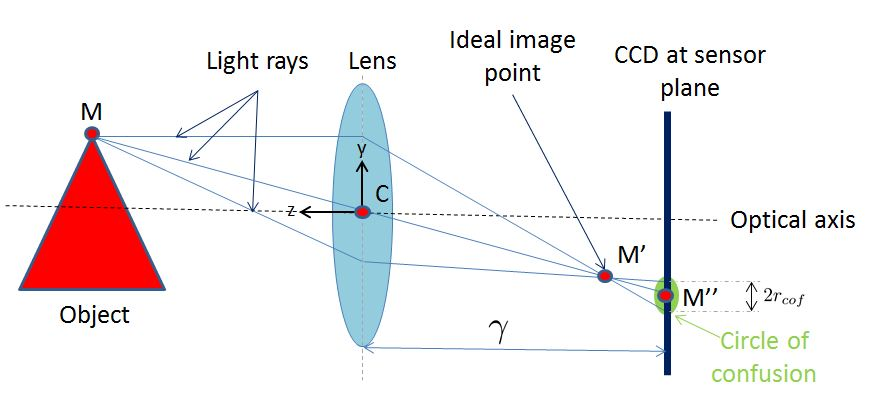
\includegraphics[scale=0.6]{Optics}
    \caption{Illustration of how light rays are manipulated by the lens}
    \label{fig:optics}
\end{figure}

% Due to the way the lens bends the light rays the image formed if the sensor plane is coincident with the resulting in an inverted image M'' (x'',y'',z'') if the sensor plane is behind the ideal image point. Since this is the most common camera configuration an inverted coordinate system is used for the sensor plane.

The thin lens equation can be stated as
\begin{equation}
\frac{1}{|CM|} + \frac{1}{CM'} = \frac{1}{\mean{f}}
\end{equation}
where $\mean{f}$ is the focal length; an inherent property of the lens. Additionally through similarity of triangles we have
\begin{align}
\frac{y}{CM} = \frac{-y'}{CM'}\\
\frac{x}{CM} = \frac{-x'}{CM'}\\
\frac{z}{CM} = \frac{-z'}{CM'}.
\end{align}
Combining these a series of equations for the ideal image point can be obtained.
\begin{align}
\label{eq:optics y'2y}
\begin{split}
x'&=\frac{-\mean{f} x}{z - \mean{f}} \\
y'&=\frac{-\mean{f} y}{z - \mean{f}} \\
z'&=\frac{-\mean{f} z}{z - \mean{f}}
\end{split}
\end{align}

\subsection{Circle of confusion}
It is impossible to align the sensor plane perfectly with the ideal image points and so the divergence of the light rays after the ideal image point causes the light rays to illuminate a circular area on the sensor plane. This blurred region is known as the circle of confusion. If this circular area is larger than the area spanned by an element of the sensor then this will result in blurring in the image as the light spills over multiple sensors. This blur could be eliminated by having the sensor plane the same distance from the lens as the the ideal image point but different points on the object will have different ideal image points.

The light rays that make up the outer perimeter of the circle of confusion are the rays that pass through the lens on the outer edges. Using these rays it is possible to determine the radius of the circle of confusion. Taking $r$ to be the radius of the lens these outer light rays pass through the midplane of the lens at $[r \cos \beta, r \sin \beta, 0]^T$ where $0<\beta<2\pi$. Using trigonometry the y components of these light rays can be related.
\begin{equation}
	\frac{y' - r \sin \beta}{z'}= \frac{y' - y''}{\gamma + z'}
\end{equation}
Th distance between the lens and the sensor plane is given by $\gamma$. The same can be done for the x component. Using this and equation \ref{eq:optics y'2y} an expression for the perimeter of the circle of confusion can be found.
\begin{equation}
\label{eq:cof}
	\begin{bmatrix}
	x'' \\
	y'' \\
	z''
	\end{bmatrix} =
	\begin{bmatrix}
	r \cos \beta + r \cos \beta \left( 1 + \frac{\gamma \left( \mean{f} - z \right)}{\mean{f} z} \right) \\
	r \sin \beta + r \sin \beta \left( 1 + \frac{\gamma \left( \mean{f} - z \right)}{\mean{f} z} \right) \\
	0
	\end{bmatrix} +
	\begin{bmatrix}
	-\frac{\gamma x}{z} \\
	-\frac{\gamma y}{z} \\
	- \gamma
	\end{bmatrix}
\end{equation}
The radius of the circle of confusion can be determine by taking the difference in the y components of $y''$ for $\beta=90 ^{\circ} $ and $\beta=270 ^{\circ}$.

\begin{align}
	2 r_{cof} &= \left[r \sin 90 ^{\circ} \left( 2 + \frac{\gamma \left( \mean{f} - z \right)}{\mean{f} z} \right) \right] - \left[r \sin 270 ^{\circ} \left( 2 + \frac{\gamma \left( \mean{f} - z \right)}{\mean{f} z} \right) \right] \\
	r_{cof}&=r \left( 1 + \frac{\gamma \left( \mean{f} - z \right)}{\mean{f}z} \right)
\end{align}

Another way that the blur can be improved is by using an aperture. An aperture is at a basic level an opaque diaphragm with a hole in it which serves to reduce the amount of light that is incident upon the sensor. Thus by blocking off the light that passed through the outer edges of the lens the aperture reduces the size of the circle of confusion by effectively reducing the radius of the lens. The aperture can be place in front or behind the lens. 

\subsection{Depth of field}
Depth of field is defined as the distance ahead and behind the object that is in focus. For a particular camera system the ideal image point of an object will fall upon the sensor plane if the object is at an ideal focal length from the lens. If the object is any closer or further from the lens it will cause a circle of confusion on the sensor plane as opposed to a point. If the circle of confusion is small enough it will not spill significant light over multiple sensors which will result in a clear image.% be interpreted as a point by the light sensor in which case it is clear in the image.

However if the circle of confusion is large enough it will cause blurring in the image. The largest circle of confusion which still results in a sharp image is referred to as the acceptable circle of confusion \cite{sutton2009image}. Thus the depth of field can be considered as the distance along the z-axis ahead or behind the ideal focus length which results in an acceptable circle of confusion.

The largest degree of freedom for a specific camera system occurs when the object is at the hyperfocal length, $H$, from the camera. The hyperfocal length is defined as the closest an object can be to the camera such that the depth of field extends to infinity behind the object. In this situation the depth of field starts at a distance of $\frac{H}{2}$. The hyperfocal length can be approximated as
\begin{equation}
	H \simeq \frac{\mean{f}^2}{2 N r_{cof}}
	\label{eq:hyperfocal}
\end{equation}
Here $N$ is given by $\frac{\mean{f}}{D_p}$ where $D_p$ is the diameter of the entrance pupil for the camera system. Letting $s$ be the distance from the camera to the object such that the camera is ideally focused at a distance $s$. The distance from the camera to the near limit of the depth of field, $D_N$, and the distance from the camera to the far limit of the depth of field, $D_F$, can be approximated.
\begin{align}
	D_N \simeq \frac{Hs}{H+s} \\
	D_F \simeq \frac{Hs}{H-s}
\end{align}
These approximations assume that the object distance is large compared to the lens focal length. The depth of field can then be determined.
\begin{equation}
	DOF = D_F - D_N = \frac{2 H s^2}{H^2 - s^2}
	\label{eq:DOF}
\end{equation}
Combining equation \ref{eq:hyperfocal} and \ref{eq:DOF} 
\begin{equation}
	DOF = \frac{4 N r_{cof} \mean{f}^2 s^2}{\mean{f}^4 - 4 N^2 r_{cof}^2 s^2}.
\end{equation}
Thus it is clear that the depth of field can be controlled by altering the focal length of the lens, by altering $N$ by changing the aperture or changing the distance between the camera and the object.

\subsection{Field of view}
\todo{viewing frustum}
The field of view is the extent of the world that the camera is capable of capturing in an image. It is quantified as the largest angle that a light ray, that is incident upon the sensor, makes with the optical axis. This angle is referred to as the angle-of-view.

Using the pinhole camera model with a distance of $L$ between the sensor and the lens and taking the lens height to be $d$ a relation for the angle-of-view, $\alpha$, can be derived using trigonometry.
\begin{align}
	\tan \left( \frac{\alpha}{2} \right) &= \frac{d}{2 L} \\
	\alpha &= 2 \arctan \left( \frac{d}{2L} \right)
\end{align}

However for the best picture quality the distance between the sensor and the lens should be equal to the focal length $f$.
\begin{equation}
	\alpha = 2 \arctan \left( \frac{d}{2f} \right)
\end{equation}

\subsection{Transformation to image plane}
The relation between an object point and the projection of the object point onto the sensor can be derived from equation \ref{eq:cof} by eliminating the circle of confusion component. Additionally when the camera system is set up properly $z'$ will be equal to $\gamma$ so that the sensor plane is approximately coincident with the ideal image points. 
\begin{equation}
\label{eq:w2i}
	\begin{bmatrix}
	x'' \\
	y'' \\
	z''
	\end{bmatrix} = 
	\begin{bmatrix}
	-\frac{\gamma}{z} & 0 & 0 \\
	0 & -\frac{\gamma}{z} & 0 \\
	0 & 0 & -\gamma
	\end{bmatrix}
	\begin{bmatrix}
	x \\
	y \\
	1
	\end{bmatrix}
\end{equation}
This equation presents two issues. Firstly the dependence of the sensor positions on $z$. Secondly all the terms in the equation have metric units whereas the image coordinate system has dimensions measured in pixels. These issues are fixed by using a homogeneous from of equation \ref{eq:w2i}.
\begin{equation}
\label{eq:w2ih}
	\alpha \begin{bmatrix}
	-x'' \\
	-y'' \\
	1
	\end{bmatrix} =
	\begin{bmatrix}
	\gamma & 0 & 0 & 0 \\
	0 & \gamma & 0 & 0 \\
	0 & 0 & 1 & 0
	\end{bmatrix}
	\begin{bmatrix}
	x \\
	y \\
	z \\
	1
	\end{bmatrix}
\end{equation}
Here $\alpha$ is a scale factor which allows for the conversion from metric units for the world coordinate system to pixels used in the sensor coordinate system. This equation is referred to as perspective projection \cite{sutton2009image}.

\subsection{Front image plane model}
A new imaging model that is often preferred for computer vision applications can be obtained by translating the sensor plane a distance of $2\gamma$ along the optical axis. In this case the sensor plane is in front of the lens. Treating the sensor coordinates $M''$ of an object as the intersection of the light ray with the sensor plane; equation \ref{eq:w2ih} remains valid for this configuration.

This imaging model is advantageous in that the sensor plane coordinates are no longer inverted. This means that the scene being imaged is also not inverted.

% \begin{itemize}
% 	\item intro
% 	\item circle of confusion
% 	\item M to M''
% 	\item aperture
% 	\item DOF
% 	\item angle of view
% 	\item pinhole inversion
% \end{itemize}

% The surfaces are convex such that diffuse light emanating from a point on an object that passes through the lens will converge and intersect at a point called the ideal imaging point. After the ideal imaging point the light rays begin to diverge again. Once this divergence occurs the image becomes inverted. The lens is placed in front of the sensor plane in an attempt to focus the light from each part of the object onto a single light sensor.

% Lenses are usually disk shaped pieces of glass with two convex surfaces. The surfaces are convex such that diffuse light emanating from a point on an object that passes through the lens will converge and intersect at a point called the ideal imaging point. After the ideal imaging point the light rays begin to diverge again. Once this divergence occurs the image becomes inverted. The lens is placed in front of the sensor plane in an attempt to focus the light from each part of the object onto a single light sensor.

% This is illustrated in figure \todo{figure}.

%  which refract light that passes through them to bring the light closer to the usually shaped such that they have convex surfaces that are shaped in such a way that light passing through the lens is refracted towards the optical axis such that  
\section{Coordinate systems}
\label{sec:coord sys}
Images are only capable of storing two dimensional information whereas we live in a three dimensional world. Thus cameras convert three dimensional information from the world coordinate system into two dimensional information in the sensor coordinate system when a picture is taken as shown in figure \ref{fig:coordsys}. The mathematical relationship between these two coordinate systems is discussed here.

\begin{figure}[h]
    \centering
    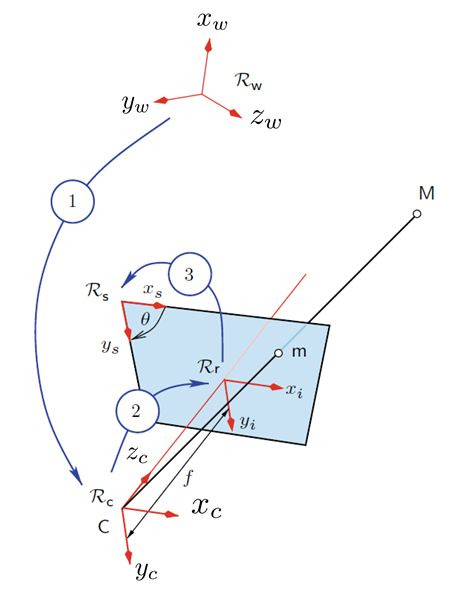
\includegraphics[scale=0.5]{CoordinateSystems}
    \caption{The conversion between coordinate systems that occurs when an image is taken}
    \label{fig:coordsys}
\end{figure}
% Throughout this project thin lenses are assumed. A thin lens is one in which its thickness is negligible in comparison with its focal length or radius of curvature. Additionally the paraxial approximation is assumed which states that light rays passing through the lens do so with a small angle to the lens's optical axis and pass through the lens close to the optical axis. This leads to the small angle approximation.
% \begin{equation}
% 	\sin(\theta) \approx \tan(\theta) \approx \theta
% \end{equation}
\todo[inline]{describe how homogeneous coordinates allow n dim vectors to be manipulated in n+1 dim space}
\subsection{Homogeneous coordinates}
It is common knowledge that any object's shape can be fully defined using distances and angles in 3D Euclidean space. However when an image is taken of this object these distances and angles become distorted. For example railway tracks consist of two beams that remain parallel to one another at a set distance apart in Euclidean space but in an image of the railway track (projective space) these beams appear to get closer and closer to one another as seen in figure \ref{fig:traintrack}. Therefore the parallelism between the beams in Euclidean space is distorted in projective space. This occurs as a result of reducing 3D information to a 2D image. \todo{add image}

\begin{figure}[h]
    \centering
    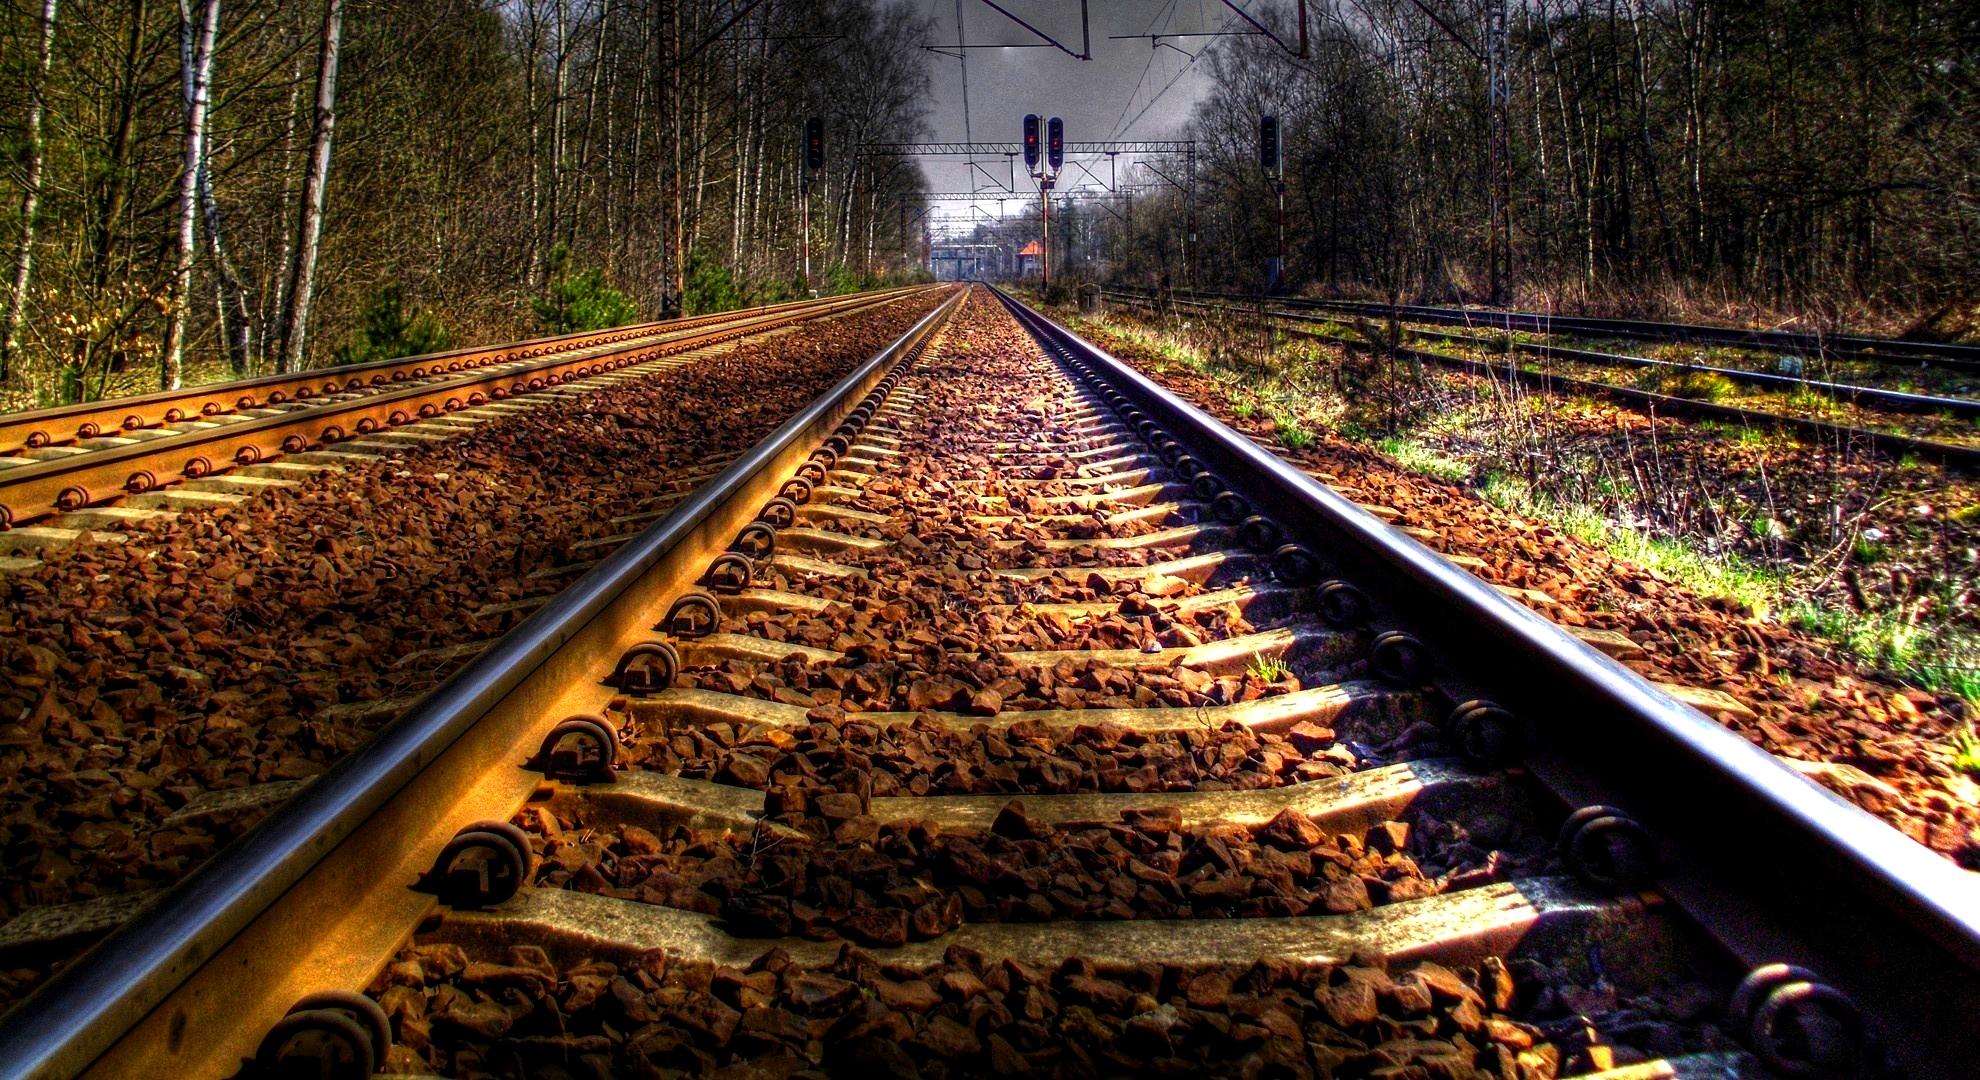
\includegraphics[scale=0.1]{TrainTrack}
    \caption{How projective space distorts parallelism present in Euclidean space}
    \label{fig:traintrack}
\end{figure}

Homogeneous coordinates make it possible to take a 3D coordinate in Euclidean space into a 4D coordinate in projective space. This is necessary since a transformation matrix for 3D coordinates that applies both rotation and translation has 4 columns and so can only be applied to a 4D coordinate. Conversion to homogeneous coordinates involves adding an additional coordinate $w$ to the coordinate vector and setting $w=1$. To convert back from homogeneous coordinates requires dividing the $x$, $y$ and $z$ coordinates by $w$ and then eliminating $w$.

\todo{do a 2D example}
% http://www.songho.ca/math/homogeneous/homogeneous.html
% http://www.tomdalling.com/blog/modern-opengl/explaining-homogenous-coordinates-and-projective-geometry/
\subsection{World to camera coordinate system}
Converting from the world coordinate system to the camera coordinate system involves rigid transformations of translation $T$ and rotation $R$. The world coordinate system is simply the coordinate system that would be used to classify the position and orientation of objects in the real world. The world coordinate systems orientation and origin is somewhat arbitrary and it is usually classified according to the object to be imaged. 

The camera coordinate system is as the name suggests fixed according to the cameras position and orientation. The camera coordinate system's z axis is the optical axis of the camera. The conversion between the two coordinate systems can be represented as
\begin{equation}
	\bm{X}_c = 
	\begin{bmatrix}
	x_c \\
	y_c \\
	z_c \\
	1
	\end{bmatrix}
	=
	\begin{bmatrix}
	r_{11} & r_{12} & r_{13} & t_1 \\
	r_{21} & r_{22} & r_{23} & t_2 \\
	r_{31} & r_{32} & r_{33} & t_3 \\
	0 & 0 & 0 & 1
	\end{bmatrix}
	\begin{bmatrix}
	x_w \\
	y_w \\
	z_w \\
	1
	\end{bmatrix} = 
	\begin{bmatrix}
	\bm{R} & \bm{T} \\
	\bm{0} & 1
	\end{bmatrix} \bm{X}_w.
\end{equation}
\todo{change T and R to lowercase}
Scaling of dimensions between the two coordinate systems also needs to be taken into account. The parameters in $\bm{R}$ and $\bm{T}$ are referred to as extrinsic parameters since they are not dependent on the camera system's hardware but rather the camera's position and orientation in the world coordinate system.

\subsection{Camera and imaging plane coordinates}
The 3D object defined in the camera coordinate system is converted to its projection on imaging plane. This conversion is from a 3D coordinate system to a 2D coordinate system as given below using homogeneous coordinates.
\begin{equation}
\label{eq:c2i}
	\bm{X}_i = \alpha
	\begin{bmatrix}
	x_i \\
	y_i \\
	1
	\end{bmatrix} 
	= 
	\begin{bmatrix}
	\gamma & 0 & 0 & 0 \\
	0 & \gamma & 0 & 0 \\
	0 & 0 & 1 & 0
	\end{bmatrix}
	\begin{bmatrix}
	x_c \\
	y_c \\
	z_c \\
	1
	\end{bmatrix}
\end{equation}
The variable $\alpha$ is an arbitrary scale factor.

\subsection{Image plane and sensor coordinates}
At this point the locations of where the light rays originating from the object will intersect the imaging plane are known. Now it is necessary to mathematically represent how the sensor would interpret these light rays incident upon the sensor into the form of pixels. In order to do this a relation between the position of a point within a coordinate system and the pixel within an image is necessary. Additionally the sensor array is not guaranteed to the orthogonal and so a skewed coordinate system must be taken into account.

The transformation from the image plane coordinate system to a temporary skewed coordinate system with an angle of $\phi$ between the two axes can be represented by
\begin{equation}
\label{eq:plane2skew}
	\begin{bmatrix}
	x_{temp} \\
	y_{temp} 
	\end{bmatrix} =
	\begin{bmatrix}
	1 & -\cot \phi \\
	0 & \frac{1}{\sin \phi}
	\end{bmatrix}
	\begin{bmatrix}
	x_i\\
	y_i
	\end{bmatrix}.
\end{equation}
It is assumed that the two principle directions in the sensor coordinate system have different scale factors, $S_x$ and $S_y$,which have units of pixels per unit length. Applying these to the coordinates calculated in equation \ref{eq:plane2skew} and accounting for the translations $\hat c_x$ and $\hat c_y$ to convert to the origin of the sensor coordinate system results in the sensor coordinates below.
\begin{equation}
	\begin{bmatrix}
	x_s \\
	y_s
	\end{bmatrix} = 
	\begin{bmatrix}
	S_x & 0\\
	0 & S_y
	\end{bmatrix}
	\begin{bmatrix}
	x_{temp}\\
	y_{temp}
	\end{bmatrix} -
	\begin{bmatrix}
	S_x \hat c_x - S_x \hat c_y \cot \phi \\
	\frac{S_y \hat c_y}{\sin \phi}
	\end{bmatrix}=
	\begin{bmatrix}
	S_x & -S_x \cot \phi \\
	0 & \frac{S_y}{\sin \phi}
	\end{bmatrix}
	\begin{bmatrix}
	x_i \\
	y_i
	\end{bmatrix} -
	\begin{bmatrix}
	S_x \hat c_x - S_x \hat c_y \cot \phi \\
	\frac{S_y \hat c_y}{\sin \phi}
	\end{bmatrix}
\end{equation}

This can be rewritten in homogeneous form so that it is consistent with equation \ref{eq:c2i}.
\begin{equation}
	\bm{X}_s = 
	\begin{bmatrix}
	x_s \\
	y_s \\
	1
	\end{bmatrix} =
	\begin{bmatrix}
	S_x & -S_x \cot \phi & -S_x \left( \hat c_x - \hat c_y \cot \phi \right) \\
	0 & \frac{S_y}{\sin \phi} & -\frac{S_y \hat c_y}{\sin \phi} \\
	0 & 0 & 1
	\end{bmatrix}
	\begin{bmatrix}
	x_i \\
	y_i \\
	1
	\end{bmatrix} =
	\bm{A} \bm{X}_i
\end{equation}
\todo{talk about these parameters being intrinsic and combine them better}

\subsection{World to sensor coordinates}
The conversions between coordinate systems described in the previous sections can be combined into one conversion from the world coordinate system to the sensor coordinate system.
\begin{equation}
	\bm{X}_s = \alpha
	\begin{bmatrix}
	x_s \\
	y_s \\
	1
	\end{bmatrix} =
	\begin{bmatrix}
	S_x & -S_x \cot \phi & -S_x \left( \hat c_x - \hat c_y \cot \phi \right) \\
	0 & \frac{S_y}{\sin \phi} & -\frac{S_y \hat c_y}{\sin \phi} \\
	0 & 0 & 1
	\end{bmatrix}
	\begin{bmatrix}
	\gamma & 0 & 0 & 0 \\
	0 & \gamma & 0 & 0 \\
	0 & 0 & 1 & 0
	\end{bmatrix}
	\begin{bmatrix}
	r_{11} & r_{12} & r_{13} & t_1 \\
	r_{21} & r_{22} & r_{23} & t_2 \\
	r_{31} & r_{32} & r_{33} & t_3 \\
	0 & 0 & 0 & 1
	\end{bmatrix}
	\begin{bmatrix}
	x_w \\
	y_w \\
	z_w \\
	1
	\end{bmatrix}
\end{equation}

This can be simplified by combining the first two matrices.
\begin{align}
	\bm{X}_s = \alpha
	\begin{bmatrix}
	x_s \\
	y_s \\
	1
	\end{bmatrix} =
	\begin{bmatrix}
	\gamma S_x & -\gamma S_x \cot \phi & -S_x \left( \hat c_x - \hat c_y \cot \phi \right) & 0\\
	0 & \frac{\gamma S_y}{\sin \phi} & -\frac{S_y \hat c_y}{\sin \phi} & 0\\
	0 & 0 & 1 & 0
	\end{bmatrix}
	\begin{bmatrix}
	r_{11} & r_{12} & r_{13} & t_1 \\
	r_{21} & r_{22} & r_{23} & t_2 \\
	r_{31} & r_{32} & r_{33} & t_3 \\
	0 & 0 & 0 & 1
	\end{bmatrix}
	\begin{bmatrix}
	x_w \\
	y_w \\
	z_w \\
	1
	\end{bmatrix}
	\label{eq:world 2 sensor cumbersome}
\end{align}

Replacing the elements of the first matrix in equation \ref{eq:world 2 sensor cumbersome} with single variables for the purposes of simplicity the equation can be rewritten as

\begin{align}
	\alpha
	\begin{bmatrix}
	x_s \\
	y_s \\
	1
	\end{bmatrix} &=
	\begin{bmatrix}
	f_x & f_s & c_x & 0\\
	0 & f_y & c_y & 0\\
	0 & 0 & 1 & 0
	\end{bmatrix}
	\begin{bmatrix}
	r_{11} & r_{12} & r_{13} & t_1 \\
	r_{21} & r_{22} & r_{23} & t_2 \\
	r_{31} & r_{32} & r_{33} & t_3 \\
	0 & 0 & 0 & 1
	\end{bmatrix}
	\begin{bmatrix}
	x_w \\
	y_w \\
	z_w \\
	1
	\end{bmatrix} \\
	&= \bm{K} \bm{V} \bm{X}_w.
	\label{eq:world 2 sensor}
\end{align}
Here the parameters relating the world coordinate system to the sensor coordinate system are separated into two matrices. The first matrix $\bm{K}$ contains the intrinsic parameters which are fixed for a specific camera. The second matrix $\bm{V}$ contains the extrinsic parameters. The extrinsic parameters change when the camera's position and orientation relative to the world coordinate system changes.
\todo{explain this better}

\section{Distortion}
Distortion refers to a collection of phenomena that cause the actual image to differ from that of the idealised image expected from the pinhole camera model. This happens because lenses cannot be manufactured and assembled perfectly and so some misalignment and defects exist in the imaging system. Therefore in order to calculate accurate displacement information the distortions must be accounted for and corrected prior to the correlation process.

Distortion can be separated into many types as done below. The overall distortion of the image can then be mathematically represented as the linear combination of the mathematical expressions for the individual types. A brief explanation of each distortion type and the equation that accounts for the distortion it creates is given below.
% https://www.lensrentals.com/blog/2010/10/the-seven-deadly-aberrations/

\subsection{Spherical distortion}
Spherical distortion is when light rays originating from a point on an object intersect at different points on the sensor plane. This is as a result of the lens not having the perfect curvature required for all the light rays to intersect at the same point on the sensor plane. It is assumed to be axis symmetric relative to the axis passing through the centre of the sensor and to be a function of the radial distance.
\begin{equation}
	\bm{D} = \kappa_1 \rho ^4 \bm{e}_r
\end{equation}
Here $\bm{e}_r$ is the radial unit vector and $\rho$ is the distance from the origin of the sensor coordinate system to the point under consideration.

\subsection{Coma distortion}
Coma distortion affects light rays that travel towards the lens at an angle to the optical axis. Light rays that go through the centre portion of lens refocus to a point on the sensor plane, whereas light rays that pass through the outer portion of the lens don't refocus fully and intersect the sensor plane further (positive coma) or closer (negative coma) to the optical axis. This results in light from a point on an object creating a comet-like shape on the sensor plane. It is corrected with the following equation.
\begin{equation}
	\bm{D} = \kappa_2 \rho^3 \cos \left( \mean{\theta} - \mean{\theta_c} \right) \bm{e}_r
\end{equation}
Here $\mean{\theta_c}$ is the orientation of the projected lens tilt angle in the sensor plane.

\subsection{Astigmatism}
Astigmatism is caused by a lens having curvature that varies when measured along perpendicular planes. For instance the vertical plane of the lens has a different curvature to the horizontal plane of the lens. The different curvatures have different focal lengths and so light passing through the vertical portion of the lens will focus at a different distance from the lens than light that passes through the horizontal portion of the lens. This results in line like blurs on the sensor plane for the curvature that is not in focus. The degree to which the astigmatism affects the image increases further away from the centre of the image.
\begin{equation}
	\bm{D} = \kappa_3 \rho^2 \cos \left( \mean{\theta} - \mean{\theta}_A \right) \bm{e}_r
\end{equation}
Where $\mean{\theta}_A$ is the orientation of the projected astigmatic plane within the sensor plane.

\subsection{Curvature of field}
Curvature of field is a distortion that results due to the curved nature of the optical elements such as the lens. As light rays pass through the lens with a small angle to the optical axis they refocus at the sensor plane. However light rays that pass through the lens at a larger angle to the optical axis refocus at a point that is closer to the lens. This results in the light rays refocusing on a curved plane much like a shallow dome. Since the sensor is planar (flat) this causes the centre of the image to be in focus while the edges of the image are not in focus.

Curvature of field is assumed to be symmetric with respect to the optical axis and to be a quadratic function of the radial position \cite{sutton2009image}.
\begin{equation}
	\bm{D}=\kappa_4 \rho^2 \bm{e}_r
\end{equation}
Here $\kappa_4$ is the amplitude of the curvature of distortion in the sensor plane measured in $\text{pixels}^{-1}$.
% https://photographylife.com/what-is-field-curvature

\subsection{Linear}
This non-symmetric distortion component is assumed to be a linear function of radial position and is dependent on the angular position \cite{sutton2009image}.
\begin{equation}
	\bm{D} = \kappa_5 \rho \cos \left( \mean{\theta} - \mean{\theta_L} \right) \bm{e}_r
\end{equation}
Here $\mean{\theta_L}$ is the angular orientation of the linear distortion axis.

\subsection{Radial}
Radial distortion is caused by the lens having different magnification levels based on the angle of the light rays to the optical axis. As a result the image can experience a decrease in magnification with increasing distance from the optical axis (barrel distortion) or the image can experience increasing magnification with increasing distance from the optical axis (pincushion distortion). This distortion is symmetric with respect to the optical axis.
\begin{equation}
	\bm{D} = \kappa_6 \rho ^3 \bm{e}_r + \kappa_7 \rho^5 \bm{e}_r + \kappa_8 \rho^7 \bm{e}_r
\end{equation}
% http://www.shariblog.com/2013/08/difference-between-barrel-pincushion-distortion/
% https://photographylife.com/what-is-distortion
\subsection{De-centering}
De-centering distortion is caused by the lens not being in perfect alignment with the rest of the camera system. Usually this type of distortion is less severe than radial or spherical distortions.
\begin{equation}
	\bm{D} = \kappa_9 \rho^2 \left[ 3 \sin \left( \mean{\theta} - \mean{\theta_d} \right) \bm{e}_r + \cos \left( \mean{\theta} - \mean{\theta_d} \right) \bm{e}_t \right]
\end{equation}
Here $\bm{e}_t$ is the tangential unit vector and $\mean{\theta_d}$ is the orientation of the axis for maximum tangential distortion.

% http://www.pcigeomatics.com/geomatica-help/concepts/orthoengine_c/Chapter_47.html
\section{Calibration}
Calibration is a necessary process that must be completed in order to extract metric information from images. The calibration process solves for parameters that define the optical characteristics of the camera, parameters that define the orientation and position of the camera coordinate system to the world coordinate system and parameters that define the distortions that must be corrected in the images. 

The parameters that define the optical characteristics and the distortions are referred to as intrinsic parameters since they are fixed for a specific camera. The parameters that describe the orientation and position of the camera within the world coordinate system are extrinsic parameters because they change if the camera is moved. \todo{explain intrinsic and extrinsic better}

Multiple methods of calibration exist however calibration using a calibration plate is used in this project since it is one of the most popular methods and making a calibration plate is relatively simple and inexpensive. Calibration for distortion parameters will not be focused on in this section. \todo{take out distortion not used}

\subsection{Inverse problem}
Calibration is essentially a method of finding the parameters that allow 3D coordinates in the world coordinate system to be accurately related to 2D coordinates in the image coordinate system. Thus the inputs, 3D world coordinates, and outputs, 2D image coordinates, needed to be used to solve for the parameters which describe the relationship between the two which constitutes an inverse problem.

Inverse problems are typlically hard to solve and calibration is no exception. In order to solve for the calibration parameters more reliably the camera model that relates world points to sensor points is broken down to the simple pinhole camera model initially in order to solve for as few parameters as possible initially. These parameters are solved for using a closed form solution which gives good estimates to the parameters. Thereafter once these parameters have been estimated the camera model is made more complex by introducing radial distortion in order to account for imperfections in the lens system of the camera. These radial parameters are first estimated and once each parameter has a corresponding estimate all the parameters are optimized in an iterative manner.

This inverse problem is sensitive to errors in the 3D world coordinates (inputs) and 2D image coordinates (outputs) used. Thus these need to be known to a high degree of accuracy in order to solve for the intrinsic and extrinsic camera parameters reliably. This is achieved by using a calibration plate.

\subsection{Calibration plate}
A calibration plate is an object with a flat surface containing a high-contrast, regular pattern. The pattern is such that it contains definitive, point-like features which can be located to a high degree of accuracy within images taken of it. For example a checker board pattern allows for accurate calculation of the points at the corners of the squares. Thus the coordinates of these point-like features on the calibration plate will be known (inputs) and the coordinates of these point-like features in the image can be determined to a high degree of accuracy (outputs).

Since images inherently contain some level of noise it is best to have an overdetermined system of equations. This is accomplished by taking multiple images of the calibration plate and changing the relative position and orientation between the calibration plate and the camera for each image. This effectively reduces the effects of noise; making the system more robust.

\subsection{Homography}
\label{sec: homography}
Homography is a transformation that can be applied to points on a plane to bring it into alignment with another plane. It is used to bring the points on the calibration plate in the world coordinate system into alignment with their location in the image in the sensor coordinate system. The transformation from world coordinates to sensor coordinates in equation \ref{eq:world 2 sensor} is a type of homography.

Treating the calibration plate such that it lies in the x-y plane of the world coordinate system; the homography, $\bm{H}$, for calibration is given by the following equation.
\begin{equation}
	\begin{bmatrix}
	x_s \\
	y_s \\
	1
	\end{bmatrix} = 
	\alpha
	\begin{bmatrix}
	f_x & f_s & c_x & 0\\
	0 & f_y & c_y & 0\\
	0 & 0 & 1 & 0
	\end{bmatrix}
	\begin{bmatrix}
	r_{11} & r_{12} & r_{13} & t_1 \\
	r_{21} & r_{22} & r_{23} & t_2 \\
	r_{31} & r_{32} & r_{33} & t_3 \\
	0 & 0 & 0 & 1
	\end{bmatrix}
	\begin{bmatrix}
	x_w \\
	y_w \\
	0 \\
	1
	\end{bmatrix} \\
\end{equation}
This can be reduced to 
\begin{align}
	\begin{bmatrix}
	x_s \\
	y_s \\
	1
	\end{bmatrix} &=
	\alpha
	\begin{bmatrix}
	f_x & f_s & c_x \\
	0 & f_y & c_y \\
	0 & 0 & 1 
	\end{bmatrix}
	\begin{bmatrix}
	r_{11} & r_{12} & t_1 \\
	r_{21} & r_{22} & t_2 \\
	r_{31} & r_{32} & t_3 
	\end{bmatrix}
	\begin{bmatrix}
	x_w \\
	y_w \\
	1
	\end{bmatrix} \\
	&= \alpha \bm{K} 
	\begin{bmatrix}
	\bm{r}_1 & \bm{r}_2 & \bm{t}
	\end{bmatrix}
	\begin{bmatrix}
	x_w \\
	y_w \\
	1
	\end{bmatrix} \\
	&= \alpha
	\begin{bmatrix}
	h_1 & h_2 & h_3 \\
	h_4 & h_5 & h_6 \\
	h_7 & h_8 & h_9
	\end{bmatrix} 
	\begin{bmatrix}
	x_w \\
	y_w \\
	1
	\end{bmatrix}
	=\alpha \bm{H} 
	\begin{bmatrix}
	x_w \\
	y_w \\
	1
	\end{bmatrix} \label{eq: homography 1}
\end{align}
Here $\bm{r}_1$ and $\bm{r}_2$ are the first and second columns of the rotation matrix. It is clear that the homography matrix contains both intrinsic and extrinsic parameters and thus it is different for each image taken of the calibration plate. Additionally note that the homography matrix is defined up to a scale factor.

%http://www.learnopencv.com/homography-examples-using-opencv-python-c/

\subsection{Estimating homography with direct linear transform}
The homographies that relate the world coordinates of the calibration plate targets to the targets in the image can be estimated using direct linear transformation \cite{zhangtut}. Equation \ref{eq: homography 1} can be written out as
\begin{align}
	x_s &= \alpha \left( h_1 x_w + h_2 y_w + h_3 \right) \label{eq: homo line 1} \\
	y_s &= \alpha \left( h_4 x_w + h_5 y_w + h_6 \right) \label{eq: homo line 2} \\
	1 &= \alpha \left( h_7 x_w + h_8 y_w + h_9 \right) \label{eq: homo line 3}.
\end{align}
The scale factor, $\alpha$, can be eliminated by dividing equations \ref{eq: homo line 1} and \ref{eq: homo line 2} by \ref{eq: homo line 3} to get
\begin{align}
	x_s \left( h_7 x_w + h_8 y_w + h_9 \right) &= \left( h_1 x_w + h_2 y_w + h_3 \right) \\
	y_s \left( h_7 x_w + h_8 y_w + h_9 \right) &= \left( h_4 x_w + h_5 y_w + h_6 \right)
\end{align}
These equations then reduce to
\begin{align}
	- h_y x_w x_s - h_8 y_w x_s + h_1 x_w + h_2 y_w +h_3 &= h_9 x_s \label{eq: solve homo 1}\\
	- h_7 x_w y_s - h_8 y_w y_s + h_4 x_w + h_5 y_w + h_6 &= h_9 y_s. \label{eq: solve homo 2}
\end{align}
In order to avoid the trivial solution where every element in the homogrpahy matrix is equal to zero; constraints need to be placed on the elements of the homography matrix. In this case the element $h_9$ is set equal to 1 however other constraints are also possible such as $h_7^2 + h_8^2 + h_9^2 = 1$. Note that if the true value of $h_9$ is close to zero then this assumption will introduce a singluarity \cite{emerging}.

Each target, having points $x_{w_i}$ and $y_{w_i}$, on the calibration plate that is captured within an image of the calibration plate, having points $x_{s_i}$ and $y_{s_i}$, provides both an equation \ref{eq: solve homo 1} and \ref{eq: solve homo 2}. These are then combined into an equation of the form
\begin{align}
	\begin{bmatrix}
	x_{w_1} & y_{w_1} & 1 & 0 & 0 & 0 & -x_{w_1} x_{s_1} & -y_{w_1} x_{s_1} \\
	0 & 0 & 0 & x_{w_1} & y_{w_1} & 1 & -x_{w_1} y_{s_1} & -y_{w_1} y_{s_1} \\
	x_{w_2} & y_{w_2} & 1 & 0 & 0 & 0 & -x_{w_2} x_{s_2} & -y_{w_2} x_{s_2} \\
	0 & 0 & 0 & x_{w_2} & y_{w_2} & 1 & -x_{w_2} y_{s_2} & -y_{w_2} y_{s_2} \\
	\vdots & \vdots & \vdots & \vdots & \vdots & \vdots & \vdots & \vdots 
	\end{bmatrix}
	\begin{bmatrix}
	h_1 \\
	h_2 \\
	h_3 \\
	h_4 \\
	h_5 \\
	h_6 \\
	h_7 \\
	h_8
	\end{bmatrix} =
	\begin{bmatrix}
	x_{s_1} \\
	y_{s_1} \\
	x_{s_2} \\
	y_{s_2} \\
	\vdots
	\end{bmatrix}
\end{align}
This overdetermined system of equations then can be used to solve for the homography matrices of each calibration image using least squares. This is the first step involved in calibration. \todo{speak about normalisation}

\subsection{Absolute conic}
\label{sec: abs conic}
As mentioned before two objects that are parallel in Euclidean space appear to intersect each other in projective space. The intersection of these two lines in projective space occurs at a point that lies on the plane at infinity. If a point lies upon the plane at infinity its $w$ is equal to zero in homogeneous coordinates.

The absolute conic lies on the plane at infinity and is defined by the set of points, $\tilde{\bm{x}}_{ac} = [x, y, z, w]^T$, that satisfies the following. 
\begin{align}
	w = 0 \\
	\bm{x}_{ac}^T \bm{x}_{ac}=x^2 + y^2 + z^2 = 0 
	\label{eq:conditions of absolute conic}
\end{align}
Here tilde is used to indicate homogeneous coordinates whereas $\bm{x}_{ac} = [x, y, z]^T$ would be the point in Euclidean space.

Thus it is the conic of purely imaginary points that lies upon the plane at infinity. The importance of the absolute conic is that it is invariant under any Euclidean transformations. In other words the relative position of the absolute conic to a moving camera is unaffected by extrinsic parameters. Consider a point $\bm{x}_{ac}$ in Euclidean space in the world coordinate system that lies on the absolute conic. It has homogeneous coordinates $\tilde{\bm{x}}_{ac}=[\bm{x}_{ac}^T, 0]^T$ in projective space. Applying a different rotation and translation to this point to obtain $\tilde{\bm{x}}_{ac}'$, which is equivalent to moving the camera in the world coordinate system, a corresponding point is obtained in the camera coordinate system.
\begin{align}
	\tilde{\bm{x}}_{ac}' &=
	\begin{bmatrix}
	\bm{R} & \bm{T} \\
	\bm{0} & 1
	\end{bmatrix}
	\tilde{\bm{x}}_{ac} =
	\begin{bmatrix}
	r_{11} & r_{12} & r_{13} & t_1 \\
	r_{21} & r_{22} & r_{23} & t_2 \\
	r_{31} & r_{32} & r_{33} & t_3 \\
	0 & 0 & 0 & 1
	\end{bmatrix}
	\begin{bmatrix}
	x_{ac} \\
	y_{ac} \\
	z_{ac} \\
	0
	\end{bmatrix} \\
	&= 
	\begin{bmatrix}
	\bm{R} \bm{x}_{ac} \\
	0
	\end{bmatrix}
\end{align}
It is clear that this point still lies on the plane at infinity since its $w$ is equal to zero. More importantly it can be proven that this point $\bm{x}_{ac}'$ is on the same absolute conic.
\begin{equation}
	\bm{x}_{ac}'^T \bm{x}_{ac}' = \left( \bm{R} \bm{x}_{ac} \right) ^T \left( \bm{R} \bm{x}_{ac} \right) = \bm{x}_{ac}^T \bm{R}^T \bm{R} \bm{x}_{ac} = \bm{x}_{ac}^T \bm{x}_{ac} = 0
\end{equation}
Thus the absolute conic is invariant to Euclidean transformations. Now consider again a point, $\bm{x}_{ac}$, lying on the absolute conic. The corresponding point, $\bm{m}_s$, in the sensor plane is given by
\begin{align}
	\tilde{\bm{m}}_s &= \frac{1}{\alpha} \bm{K} 
	\begin{bmatrix}
	\bm{R} & \bm{T} \\
	\bm{0} & 1
	\end{bmatrix}
	\begin{bmatrix}
	\bm{x}_{ac} \\
	0
	\end{bmatrix} = \frac{1}{\alpha} \bm{K}
	\begin{bmatrix}
	\bm{R} \bm{x}_{ac} \\
	0
	\end{bmatrix} \\
	\therefore \bm{m}_s &= \frac{1}{\alpha} \bm{K} \bm{R} \bm{x}_{ac}.
\end{align}
Checking whether this point satisfies equation \ref{eq:conditions of absolute conic} results in
\begin{equation}
	\bm{m}_s^T \bm{K}^{-T} \bm{K}^{-1} \bm{m}_s = \frac{1}{\alpha^2} \bm{x}_{ac}^T \bm{R}^T \bm{R} \bm{x}_{ac} = \frac{1}{\alpha^2} \bm{x}_{ac}^T \bm{x}_{ac} = 0
\end{equation}
Thus the image of the absolute conic is itself an imaginary conic. The image of the absolute conic is defined by $\bm{K}^{-T} \bm{K}^{-1}$ \cite{luong1997self}. Thus since the image of the absolute conic is dependent only on intrinsic camera parameters it can be used to solve for the intrinsic camera parameters.

% http://www.cs.unc.edu/~marc/tutorial/node87.html
\subsection{Constraints on intrinsic parameters}
\label{sec: intrinsic constraints}
According to Zhang \cite{emerging} there are two constraints placed upon the intrinsic parameters of the camera. These are important later on in the solving for these intrinsic parameters. The plane of the calibration plate in the camera coordinate system is given by \cite{emerging} 
\begin{equation}
	\begin{bmatrix}
	\bm{r}_3 \\
	\bm{r}_3^T \bm{t}
	\end{bmatrix}^T
	\begin{bmatrix}
	x \\
	y \\
	z \\
	w
	\end{bmatrix} = 0.
\end{equation}
Here $w$ is zero for points on the plane at infinity and one for those that are not. This plane intersects the plane at infinity on a line and it happens that $[\bm{r}_1^T, 0]^T$ and $[\bm{r}_2^T, 0]^T$ are points on this line \cite{emerging}. Thus it is known that any point on this line, $x_c^{\infty}$, is a linear combination of these two points.
\begin{equation}
	x_c^{\infty} = a \begin{bmatrix}
	\bm{r}_1 \\
	0
	\end{bmatrix} + b
	\begin{bmatrix}
	\bm{r}_2 \\
	0
	\end{bmatrix} =
	\begin{bmatrix}
	a \bm{r}_1 + b \bm{r}_2 \\
	0
	\end{bmatrix}
\end{equation}
Now assume that this point, $x_c^{\infty}$, lies on the absolute conic. Then this point must satisfy equation \ref{eq:conditions of absolute conic}. This would require that $a^2+b^2=0$ which results in the solution $b=\pm a i$, where $i=\sqrt{-1}$. As a result it can be seen that the two points along this line intersect the absolute conic at
\begin{equation}
	x_c^{\infty} = a 
	\begin{bmatrix}
	\bm{r}_1 \pm i \bm{r_2} \\
	0
	\end{bmatrix}.
\end{equation}
Since these points lie on the absolute conic they are invariant under Euclidean transformations. Their projection, up to a scale factor, in the sensor coordinate system is given by
\begin{equation}
	x_s^{\infty} = \bm{K} \left( \bm{r}_1 \pm \bm{r}_2 \right) = \bm{h}_1 \pm i \bm{h}_2.
\end{equation}
Substituting these points into equation \ref{eq:conditions of absolute conic} results in
\begin{equation}
	\left( \bm{h}_1 \pm i \bm{h}_2 \right)^T \bm{K}^{-T} \bm{K}^{-1} \left( \bm{h}_1 \pm i \bm{h}_2 \right) = 0.
\end{equation}
Requiring both the imaginary and real parts of this equation to equal zero results in two constraints on the intrinsic camera parameters.
\begin{align}
\label{eq:intrinsic constraints}
	\bm{h}_1^T \bm{K}^{-T} \bm{K}^{-1} \bm{h}_2 &= 0 \\
	\bm{h}_1^T \bm{K}^{-T} \bm{K}^{-1} \bm{h}_1 &= \bm{h}_2^T \bm{K}^{-T} \bm{K}^{-1} \bm{h}_2
\end{align}

\subsection{Intrinsic parameters and the absolute conic}
\label{sec: parameters and the absolute conic}
An homography, $\bm{H}$, between the calibration plate and the image of the calibration plate can be estimated. This homography can then be used to solve for the image of the absolute conic. Once the image of the absolute conic is known it can be used to solve for the intrinsic camera parameters. The image of the absolute conic can be represented as
\begin{equation}
	\bm{B} = \bm{K}^{-T} \bm{K}^{-1} = 
	\begin{bmatrix}
	b_{11} & b_{12} & b_{13}\\
	b_{12} & b_{22} & b_{23} \\
	b_{13} & b_{23} & b_{33}
	\end{bmatrix}
\end{equation}
Since $\bm{B}$ is symmetric its contents can be represented by a 6D vector $\bm{b}=[b_{11} b_{12} b_{22} b_{13} b_{23} b_{33}]^T$. Let $\bm{h}_i = [h_{i1} h_{i2} h_{i3}]^T$ to be the i\textsuperscript{th} column of $\bm{H}$. Then
\begin{equation}
	\bm{h}_I^T \bm{B} \bm{h}_j = \bm{v}_{ij} \bm{b}
\end{equation}
where 
\begin{equation}
	\bm{v}_{ij} = [ h_{i1} h_{j1}, h_{i1} h_{j2} + h_{i2} h_{j1}, h_{i2} h_{j2}, h_{i3} h_{j1} + h_{i1} h_{j3}, h_{i3} h_{j2} + h_{i2} h_{j3}, h_{i3} h_{j3}]^T.
\end{equation}
Then equation \ref{eq:intrinsic constraints} can be rewritten as 
\begin{equation}
	\begin{bmatrix} 
	\bm{v}_{12}^T \\
	( \bm{v}_{11} - \bm{v}_{22})^T
	\end{bmatrix} \bm{b} = \bm{0}
\end{equation}
A separate version of this equation exist for each image taken of the calibration plate and these equations can be stacked, in $\bm{V}$, to give
\begin{equation}
	\bm{V}\bm{b}=\bm{0}.
\end{equation}
The solution for $\bm{b}$, up to a scale factor $\lambda$, is known to be the eigenvector of $\bm{V}^T\bm{V}$ associated with the smallest eigenvalue \cite{emerging}. Once b has been determined it can be used to determine the intrinsic parameters of matrix $\bm{K}$. The relation between $\bm{B}$ and $\bm{K}$ is $\bm{B}=\lambda \bm{K}^{-T} \bm{K}^{-1}$. The intrinsic parameters are determined as follows.
\begin{align}
	c_y &= (b_{12} b_{13} - b_{11} b_{23})/(b_{11} b_{22} - b_{12}^2) \\
	\lambda &= b_{33} -(b_{13}^2 + c_y(b_{12} b_{13} - b_{11} b_{23}))/b_{11}\\
	f_x &= \sqrt{\frac{\lambda}{b_{11}}} \\
	f_y &= \sqrt{\frac{\lambda b_{11}}{b_{11} b_{22} - b_{12}^2}} \\
	f_s &= \frac{-b_{12} f_x^2 f_y}{\lambda} \\
	c_x &= \frac{f_s c_y}{f_y} - \frac{b_{13} f_x^2}{\lambda}
\end{align}
Thereafter the extrinsic parameters can be determined.
\begin{align}
	\bm{r}_1 &= \lambda \bm{K}^{-1} \bm{h}_1 \\
	\bm{r}_2 &= \lambda \bm{K}^{-1} \bm{h}_2 \\
	\bm{r}_3 &= \bm{r}_1 \times \bm{r}_2 \\
	\bm{T} &= \lambda \bm{K}^{-1} \bm{h}_3
\end{align}
At this point it is necessary to incorporate distortions and use them to find better approximations for the intrinsic and extrinsic parameters.

\todo{this section is too close to the paper} %a fleixible new technique and reading 1
% by which the optical characteristics of a camera and the relation between its coordinate system and the world coordinate system are determined. It is performed in order to be able to extract \hl{metric} information from images accurately.

\subsection{Closed form solution}
Sections \ref{sec: homography} throught to \ref{sec: parameters and the absolute conic} illustrate that estimates to the intrinsic and extrinsic parameters can be obtained by first determining the homographies for each calibration image, then these can be used to determine the image of the abolute conic which in turn can be used to determine the intrinsic and extrinsic camera parameters. This is closed form solution is the first part of the calibration process

put inverse problem in calibration plate section

explain homography and absolute conic

then explain closed form solution and optimization - give closed form and explain optimization


\subsection{Distortion in Calibration}
The closed form solution given above does not take distortion into account since it is based on the pinhole camera model. It is only once the closed form solution to the extrinsic and intrinsic parameters is optimised that distortion can be accounted for during the calibration process. As already presented, there are many types of distortion that occur when an image is taken. However it is seldom possible to take all of these distortion types into account since the more distortion paramters introduced into the camera model; the more likely the optimization process becomes unstable.

It has been found \todo{add reference for this} that good calibration results can be achieved by taking only radial distortion into accound during calibration \cite{tsai1987versatile,wei1994implicit}. This is beneficial since it is possible to solve for initial guesses to the radial distortion parameters which helps the optimisation process to avoid local minima as a result of the distortion parameters used.

The distortion applied to the points on the image plane is of the form
\begin{align}
	\begin{bmatrix}
	x_{i_{distorted}} \\
	y_{i_{distorted}}
	\end{bmatrix} &=
	1 + k_1 r^2 + k_2 r^4
	\begin{bmatrix}
	x_i \\
	y_i
	\end{bmatrix}\\
	\text{where} \quad \quad r &= \sqrt{x_i^2 + y_i^2}.
\end{align}

At this point the intrinsic and extrinsic parameters have been determined using the pinhole camera model and the error between the predicted calibration plate targets and the actual location of these in the images is attributed to radial distortion \cite{zhangtut}. This error is represented as
\begin{equation}
	d_1 = x_{s_{actual}} - x_{s_{calculated}}
\end{equation}

An undistorted point, $x_i$ is distorted to point $\tilde{x_i}$ according to
\begin{align}
	\tilde{x_i} &= u_c + (x_i-u_c)*(1 + k1 r^2 + k2 r^4) \\
	&= u_c + x_i - u_c + (x_i-u_c)*(1 + k1 r^2 + k2 r^4) \\
	&= x_i + (x_i-u_c)*(1 + k1 r^2 + k2 r^4) \\
	&= x_i + d_{2_i}
\end{align}

The distortion parameters can be estimated by minimizing the difference between $d_1$ and $d_2$. Thus the least squares solution to the overdetermined system is what is needed.


\section{Displacement fields}
In this section some displacement fields are presented in order to illustrate what information DIC and DVC are capable of extracting from image sets.

\subsection{DIC displacement fields}
The figures below show the displacement fields in the region of the crack of a compact tension sample as it is loaded in the y-direction. As such the x-displacement magnitudes are at most 10 \% of the displacements in the y-direction. It becomes clear in analysing these figures that the displacement fields determined by DIC are quite intuitive and can be easily interpreted to understand the deformation that a specimen has undergone.

Additionally these images illustrate the full-field nature of the displacement data that DIC is capable of determining. This coupled with its high accuracy and high spatial resolution makes DIC a very attractive displacement measurement tool.

\begin{figure}[h]
    \centering
    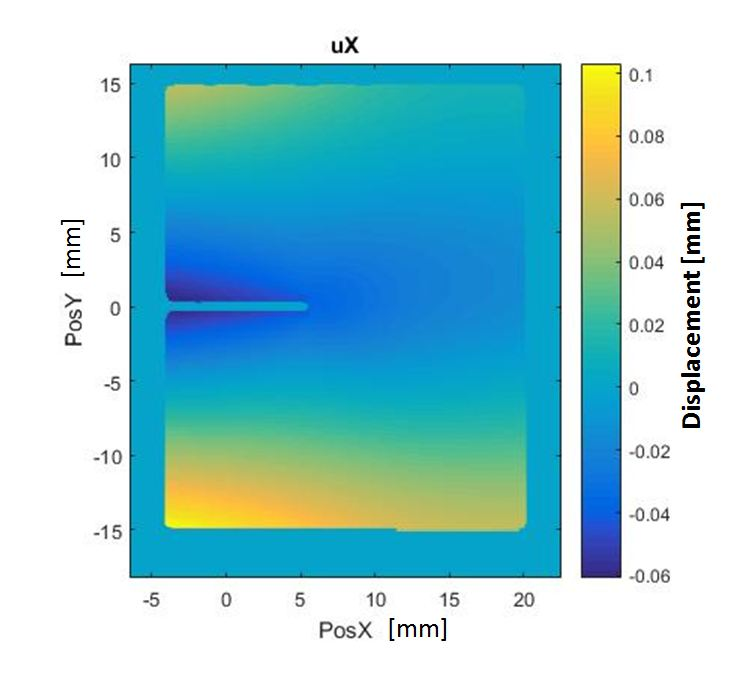
\includegraphics[scale=0.4]{DICuyx}
    \caption{X-direction displacement field of a compact tension specimen (DIC)}
    \label{fig:DICUX}
\end{figure}

\begin{figure}[h]
    \centering
    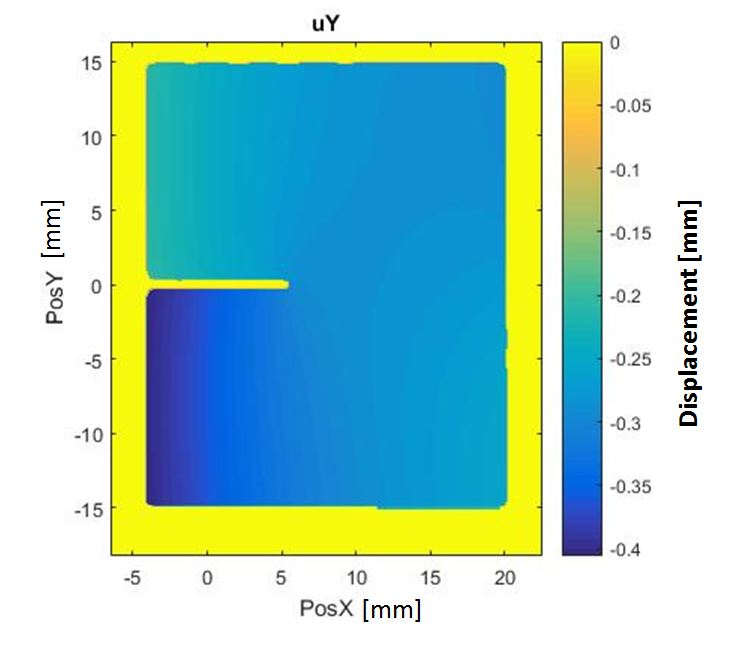
\includegraphics[scale=0.4]{DICuy}
    \caption{Y-direction displacement field of a compact tension specimen (DIC)}
    \label{fig:DICUY}
\end{figure}

\subsection{DVC displacement fields}
DIC displacement fields consist of x and y displacements of points defined in two dimensions. This is because DIC only captures the deformation on the surface of the specimen. However DVC displacement fields consist of x, y and z displacements of points defined in three dimensions. This is because DVC captures deformation information through the thickness of the specimen.

As such in order to visualise DVC displacement fields a plane through the thickness (or on the surface) of the specimen must be chosen. Then the displacements can be visualised on this plane. This plane can then be moved through the thickness of the specimen in order to determine how the displacement fields differ in that direction. 

This is illustrated in figures \ref{fig:DVC1} and \ref{fig:DVC2} by the change in location of the crack front. These figures show the z direction displacement fields of a specimen in the x-y plane at two different heights in the z direction. This is a rectangular specimen that contains a crack front which is not perpendicular to any of the specimens surfaces. These two figures show how the x-y position of the crack front changes with a change in the z position. Thus DVC allows for more of the materials response to be captured.

\begin{figure}[h]
    \centering
    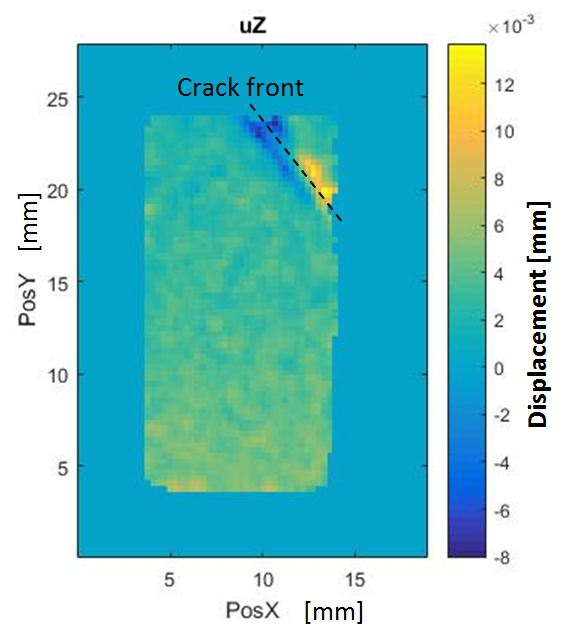
\includegraphics[scale=0.4]{DVC3}
    \caption{Z-direction displacement field on the x-y plane at a height of 13.95 mm in the z direction (DVC)}
    \label{fig:DVC1}
\end{figure}

\begin{figure}[h]
    \centering
    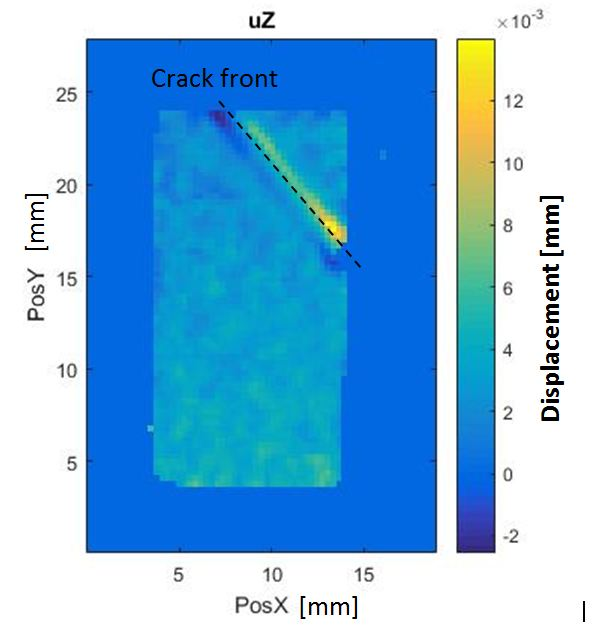
\includegraphics[scale=0.4]{DVC4}
    \caption{Z-direction displacement field on the x-y plane at a height of 15.45 mm in the z direction (DVC)}
    \label{fig:DVC2}
\end{figure}



% The location of this crack front is highlighted in the two images and it can be different at the two different heights 

% DVC displacement fields are very similar to DIC displacement fields in appearance however the difference lies in that DVC computes displacement fields through the thickness of the specimen whereas DIC only presents the displacement data for the specimens surface. 

% allow the user to quickly see what deformation a specimen underwent.

% The x-displacement is almost uniform in the horizontal direction 

% full field
% spatial resolution 
% accuracy
% visulisation 
